%-------------------------------------------------------------------------------
%                      Template Naskah Skripsi
%               	Berdasarkan format JTETI FT UGM
% 						(c) @gunturdputra 2014
%-------------------------------------------------------------------------------

%Template pembuatan naskah skripsi.
\documentclass{jtetiskripsi}

%Untuk prefiks pada daftar gambar dan tabel
\usepackage[titles]{tocloft}
\renewcommand\cftfigpresnum{Gambar\  }
\renewcommand\cfttabpresnum{Tabel\   }

%Untuk hyperlink dan table of content
\usepackage[hidelinks]{hyperref}
\newlength{\mylenf}
\settowidth{\mylenf}{\cftfigpresnum}
\setlength{\cftfignumwidth}{\dimexpr\mylenf+2em}
\setlength{\cfttabnumwidth}{\dimexpr\mylenf+2em}

%Untuk Bold Face pada Keterangan Gambar
\usepackage[labelfont=bf]{caption}

%Untuk caption dan subcaption
\usepackage{caption}
\usepackage{subcaption}

%pdf
\usepackage{pdfpages}

%table
\usepackage{array}
\usepackage{longtable}
\newcolumntype{P}[1]{>{\centering\arraybackslash}p{#1}}
\usepackage{graphics}
\usepackage{wrapfig}

%bibliography
\usepackage[
  style=authoryear-icomp,
  maxcitenames=1,
  isbn=false,
  doi=false,
  url=false,
  autolang=other,
  hyperref=true,
  sortcites=true,
  bibwarn=true,
  firstinits=true,
  autolang=other,
]{biblatex}
\DefineBibliographyStrings{english}{%
  andothers = {dkk\adddot,\addspace},
}
\DeclareFieldFormat{citehyperref}{%
  \DeclareFieldAlias{bibhyperref}{noformat}% Avoid nested links
  \bibhyperref{#1}}

\DeclareFieldFormat{textcitehyperref}{%
  \DeclareFieldAlias{bibhyperref}{noformat}% Avoid nested links
  \bibhyperref{%
    #1%
    \ifbool{cbx:parens}
      {\bibcloseparen\global\boolfalse{cbx:parens}}
      {}}}

\savebibmacro{cite}
\savebibmacro{textcite}

\renewbibmacro*{cite}{%
  \printtext[citehyperref]{%
    \restorebibmacro{cite}%
    \usebibmacro{cite}}}

\renewbibmacro*{textcite}{%
  \ifboolexpr{
    ( not test {\iffieldundef{prenote}} and
      test {\ifnumequal{\value{citecount}}{1}} )
    or
    ( not test {\iffieldundef{postnote}} and
      test {\ifnumequal{\value{citecount}}{\value{citetotal}}} )
  }
    {\DeclareFieldAlias{textcitehyperref}{noformat}}
    {}%
  \printtext[textcitehyperref]{%
    \restorebibmacro{textcite}%
    \usebibmacro{textcite}}}
\addbibresource{daftar-pustaka.bib}

%equation
\usepackage{amsmath}

%algorithm & syntax
\usepackage{algorithm}
\usepackage{algpseudocode}
\algnewcommand\algorithmicforeach{\textbf{for each:}}
\algnewcommand\ForEach{\item[ \algorithmicforeach]}
\algdef{SE}[DOWHILE]{Do}{doWhile}{\algorithmicdo}[1]{\algorithmicwhile\ #1}%
\newenvironment{conditions}
  {\par\vspace{\abovedisplayskip}\noindent\begin{tabular}{>{$}l<{$} @{${}={}$} l}}
  {\end{tabular}\par\vspace{\belowdisplayskip}}

%code
\usepackage{listings}
\usepackage{xcolor}
\definecolor{codegreen}{rgb}{0,0.6,0}
\definecolor{codegray}{rgb}{0.5,0.5,0.5}
\definecolor{codepurple}{rgb}{0.58,0,0.82}
\lstdefinestyle{mystyle}{
    commentstyle=\color{codegreen},
    keywordstyle=\color{magenta},
    numberstyle=\tiny\color{codegray},
    stringstyle=\color{codepurple},
    basicstyle=\ttfamily\footnotesize,
    frame=single,
    breakatwhitespace=false,
    breaklines=true,
    captionpos=b,
    keepspaces=true,
    numbersep=5pt,
    showspaces=false,
    showstringspaces=false,
    showtabs=false,
    tabsize=2
}
\lstset{style=mystyle}
\makeatletter
\def\thechapter{\@Roman\c@chapter}
\AtBeginDocument{%
  \def\thelstlisting{\@arabic\c@chapter.\@arabic\c@lstlisting}}
\makeatother


%-----------------------------------------------------------------
%Disini awal masukan untuk data proposal skripsi
%-----------------------------------------------------------------
\titleind{Estimasi Panjang dan Berat Ikan Menggunakan Harris-Corners Detectors}

\fullname{Prabowo Darmawi}

\idnum{1313619001}

\approvaldate{}

\degree{Sarjana Ilmu Komputer}

\yearsubmit{2024}

\program{Ilmu Komputer}

\dept{Ilmu Komputer}

\firstsupervisor{Muhammad Eka Suryana, M. Kom.}
\firstnip{198512232012121002}

\secondsupervisor{Med Irzal, M. Kom.}
\secondnip{197706152003121001}

%-----------------------------------------------------------------
%Disini akhir masukan untuk data proposal skripsi
%-----------------------------------------------------------------

\tolerance=1
\emergencystretch=\maxdimen{}
\hyphenpenalty=10000
\hbadness=10000

\begin{document}

\cover{}
%-----------------------------------------------------------------

%-----------------------------------------------------------------
%Disini akhir masukan untuk muka skripsi
%-----------------------------------------------------------------

%\chapter*{\centering{\large{LEMBAR PENGESAHAN}}}
\thispagestyle{empty} {\bf }Dengan ini saya mahasiswa Fakultas
Matematika dan Ilmu Pengetahuan Alam, Universitas Negeri Jakarta

\vskip3mm

\begin{tabular}{ll}
  Nama & : Prabowo Darmawi \\
  No. Registrasi & : 1313619001 \\
  Program Studi & : Ilmu Komputer \\
  Judul & : Penghitungan Panjang Dan Berat Ikan \\ & \hspace{0.2cm}
  Menggunakan Harris-Corners Detection \\
\end{tabular}

\vskip3mm

\noindent \hskip10mm Menyatakan bahwa proposal ini telah siap diajukan untuk seminar pra skripsi.
%\begin{center}
%Menyatakan bahwa skripsi ini telah siap diajukan untuk sidang skripsi.
%\end{center}



\begin{center}
\vskip3mm

Menyetujui,

\vskip3mm
\begin{spacing}{1.25}

\begin{tabular}{ccc}
  \hskip-2mm Dosen Pembimbing I & \qquad \qquad \qquad \qquad \qquad & \hskip-6mm Dosen Pembimbing II \\
   &  &  \\
   &  &  \\
   &  &  \\
   &  &  \\
  \hskip-2mm \underline{\textbf{Muhammad Eka Suryana, M.Kom}} &  & \hskip-6mm \underline{\textbf{Med
  Irzal, M.Kom}} \\
  \hskip-2mm NIP. 19770615 200312 1 001 &  & \hskip-6mm NIP. 19851223 201212 
  1 002	 \\
\end{tabular}
\end{spacing}
\end{center}
\vskip3mm
\begin{center}
Mengetahui, \\
Koordinator Program Studi Ilmu Komputer
\end{center}
\begin{spacing}{1.25}
{ \ }
\\
\\
{ \ }\begin{center}
\underline{\textbf{Dr. Ria Arafiyah, M.Si}} \\
{NIP. 19751121 200501 2 004}
\end{center}
\end{spacing} 

\chapter*{\centering{\large{KATA PENGANTAR}}}

Puji syukur penulis panjatkan ke hadirat Allah SWT, karena dengan rahmat dan
karunia-Nya, penulis dapat menyelesaikan proposal skripsi yang berjudul
\textit{Penghitungan Panjang dan Berat Ikan dengan Menggunakan Harris-Corner Detection}.

Keberhasilan dalam penyusunan proposal skripsi ini tidak lepas dari bantuan
berbagai pihak yang telah tulus dan ikhlas memberikan masukan guna sempurnanya proposal skripsi ini. Dalam kesempatan ini, dengan
kerendahan hati penulis mengucapkan banyak terima kasih kepada:

\begin{enumerate}

	\item{Yth. Para petinggi di lingkungan FMIPA Universitas Negeri Jakarta.}
	\item{Yth. Ibu Dr. Ria Arafiyah, M.Si selaku Koordinator Program Studi Ilmu
		Komputer.}
	\item{Yth. Bapak Muhammad Eka Suryana, M.Kom selaku Dosen Pembimbing I yang
		telah membimbing, mengarahkan, serta memberikan saran dan koreksi terhadap
		proposal skripsi ini.}
	\item{Yth. Bapak Med Irzal, M.Kom selaku Dosen Pembimbing II yang telah
		membimbing, mengarahkan, serta memberikan saran dan koreksi terhadap
		proposal skripsi ini.}
	\item{Kedua orang tua dan adik penulis yang telah mendukung dan memberikan 
		semangat serta doa untuk penulis.}
	\item{Teman-teman Program Studi Ilmu Komputer 2019 yang telah memberikan 
		dukungan dan memiliki andil dalam penulisan proposal skripsi ini.}
	
\end{enumerate}

Penulis menyadari bahwa penyusunan proposal skripsi ini masih jauh dari sempurna
karena keterbatasan ilmu dan pengalaman yang dimiliki. Oleh karenanya, kritik
dan saran yang bersifat membangun akan penulis terima dengan senang hati. 

Akhir kata, penulis berharap tugas akhir ini bisa bermanfaat bagi semua pihak baik itu bagi FMIPA Universitas Negeri Jakarta, teman-teman dari program studi Ilmu
Komputer Universitas Negeri Jakarta dan para pembaca sekalian, khususnya penulis sendiri.

Semoga Allah SWT senantiasa membalas kebaikan semua pihak yang telah membantu penulis dalam menyelesaikan proposal skripsi ini.

\vspace{4cm}

\begin{tabular}{p{7.5cm}c}
	&Jakarta, \\
	&\\
	&\\
	&\\
	&Prabowo Darmawi
\end{tabular}

\singlespacing{}
\tableofcontents{}
\addcontentsline{toc}{chapter}{DAFTAR ISI}
\listoffigures{}
\addcontentsline{toc}{chapter}{DAFTAR GAMBAR}
\listoftables{}
\addcontentsline{toc}{chapter}{DAFTAR TABEL}

\begin{counterpage}
\end{counterpage}
%Disini awal masukan untuk Bab
%-----------------------------------------------------------------

\onehalfspacing{}
%!TEX root = ./template-skripsi.tex
%-------------------------------------------------------------------------------
% 								BAB I
% 							LATAR BELAKANG
%-------------------------------------------------------------------------------

\chapter{PENDAHULUAN}

\section{Latar Belakang Masalah}

Indonesia merupakan negara kepulauan dengan kekayaan hayati yang melimpah, salah satunya adalah ikan yang menjadi sumber pangan utama masyarakat. Budidaya ikan di Indonesia terus berkembang untuk memenuhi kebutuhan konsumsi dan permintaan pasar, baik sebagai bahan pangan maupun ikan hias. Salah satu aspek penting dalam budidaya ikan adalah pengukuran panjang dan berat ikan, yang berperan dalam pemantauan pertumbuhan, penentuan dosis pakan, serta penentuan harga jual.

Namun, proses pengukuran panjang dan berat ikan di lapangan umumnya masih dilakukan secara manual, yaitu dengan menimbang dan mengukur satu per satu menggunakan alat ukur konvensional (\cite{Amri2020}). Cara ini tidak efisien, memakan waktu lama, dan berpotensi menimbulkan stres pada ikan sehingga dapat mempengaruhi kualitas dan pertumbuhan ikan. Selain itu, metode manual hanya memberikan estimasi jumlah atau berat secara keseluruhan, tanpa informasi detail mengenai distribusi ukuran ikan dalam satu populasi.

Seiring perkembangan teknologi, pengolahan citra digital menawarkan solusi otomatis untuk mengukur panjang dan berat ikan secara cepat dan akurat. Salah satu metode yang dapat digunakan adalah deteksi titik sudut (\emph{corner detection}) pada citra ikan. Titik sudut pada tubuh ikan, seperti ujung kepala dan ekor, dapat digunakan sebagai acuan untuk mengukur panjang ikan secara otomatis dari citra (\cite{Harris2013}). Dengan mengetahui panjang ikan, berat ikan juga dapat diestimasi menggunakan rumus atau model regresi yang sesuai (\cite{Diansari2013}).

Metode \emph{Harris-Corner Detection} merupakan salah satu algoritma deteksi sudut yang banyak digunakan karena kestabilannya terhadap rotasi, noise, dan efisiensi komputasi (\cite{Harris2013}). Dengan menerapkan metode ini pada citra ikan, sistem dapat secara otomatis mendeteksi titik-titik sudut penting, sehingga proses pengukuran panjang dan estimasi berat ikan dapat dilakukan secara digital, cepat, dan minim kontak langsung dengan ikan.

Berbagai penelitian sebelumnya telah mengembangkan metode untuk mendeteksi atau melacak ikan, seperti penggunaan metode GMM dan Kalman Filter untuk pelacakan gerakan (Alim, 2021), serta GrabCut untuk pemisahan objek dari latar belakang (Nugraha, 2022). Namun, metode-metode tersebut umumnya hanya fokus pada deteksi keberadaan ikan atau pelacakan pergerakan, dan belum secara langsung mengekstraksi fitur geometris seperti panjang dan berat ikan.

Di sisi lain, metode seperti SIFT (\emph{Scale Invariant Feature Transform}) (\cite{Lowe2004}) memang kuat terhadap perubahan skala dan rotasi, namun proses perhitungannya relatif kompleks dan memerlukan waktu komputasi lebih tinggi. Untuk kasus estimasi bentuk linear seperti panjang dan lebar, pendekatan berbasis deteksi sudut seperti \emph{Harris-Corner Detection} terbukti lebih efisien dan akurat dalam mendeteksi titik-titik sudut penting pada citra (\cite{Harris2013}). \emph{Harris-Corner Detection} memberikan kestabilan terhadap rotasi dan noise lokal serta memiliki struktur komputasi yang lebih ringan dibanding SIFT, sehingga cocok untuk diterapkan dalam sistem real-time atau perangkat keras terbatas.

Oleh karena itu, penelitian ini bertujuan untuk membangun sistem pengukuran panjang dan estimasi berat ikan berbasis citra digital menggunakan metode \emph{Harris-Corner Detection}. Diharapkan sistem ini dapat membantu pembudidaya ikan dalam melakukan monitoring pertumbuhan ikan secara efisien dan akurat, serta mendukung pengambilan keputusan dalam manajemen budidaya.

\section{Rumusan Masalah}
Berdasarkan pemaparan masalah di atas, perumusan masalah dalam penelitian ini adalah \textbf{“Bagaimana cara mengukur panjang serta menghitung berat ikan menggunakan metode \emph{Harris-Corner Detection}?”}

\section{Batasan Masalah}
\begin{enumerate}
	\item Sistem hanya menghitung panjang dan berat ikan dengan menggunakan \emph{Harris-Corners Detection}. 
	\item Jenis Ikan yang digunakan adalah ikan lele, ikan mas, dan ikan nila.
	\item Sumber gambar berupa dataset yang diambil langsung dari lapangan.
	\item Dataset telah dihilangkan latar belakangnya dan digantikan dengan warna solid hitam.
	\item Citra yang digunakan hanya citra tampak samping. 
	\item Bahasa Pemrograman menggunakan Python 3 atau lebih baru. 
\end{enumerate}
	
\section{Tujuan Penelitian}
	Tujuan dari Penelitian adalah Membangun sistem berbasis citra digital untuk mengestimasi panjang dan berat ikan menggunakan deteksi titik sudut dengan menggunakan metode \emph{Harris-corner detection}. 

\section{Manfaat Penelitian}
\begin{enumerate}
	\item Bagi penulis
	 Memperoleh gelar sarjana dalam bidang Ilmu Komputer, dan menambah pengalaman dalam pembangunan sebuah sistem komputer untuk aplikasi dunia nyata, serta pengetahuan tentang pendeteksian sudut atau \emph{corner} dari \emph{Harris-corner Detection}. 

		
	\item Bagi Program Studi Ilmu Komputer
	Penelitian "Penghitungan Panjang dan Berat Ikan Menggunakan Harris-Corners Detection" dapat dijadikan sebagai referensi dan menambah wawasan mahasiswa dan sivitas akademika Ilmu Komputer Universitas Negeri Jakarta.

\end{enumerate}

% Baris ini digunakan untuk membantu dalam melakukan sitasi
% Karena diapit dengan comment, maka baris ini akan diabaikan
% oleh compiler LaTeX.
\begin{comment}
\bibliography{daftar-pustaka}
\end{comment}

%!TEX root = ./template-skripsi.tex
%-------------------------------------------------------------------------------
%                            BAB II
%                          KAJIAN TEORI
%-------------------------------------------------------------------------------

\chapter{KAJIAN PUSTAKA}

\section{Pengertian Deteksi Fitur}
  Deteksi fitur adalah salah satu teknik penting dalam pengolahan citra digital yang digunakan untuk mengekstraksi informasi spesifik dari gambar. 
Fitur pada citra dapat berupa titik sudut (corner), tepi (edge), atau pola tertentu yang dapat digunakan untuk mengidentifikasi karakteristik objek di dalam gambar. 
Deteksi fitur sangat penting karena fitur-fitur ini sering kali tidak terpengaruh oleh perubahan pencahayaan, rotasi, atau skala, sehingga dapat digunakan untuk berbagai aplikasi seperti pemetaan, pengenalan objek, dan pencocokan gambar.

\section{\emph{Harris-Corner Detection}}
  \emph{Harris-Corner Detection} merupakan salah satu dari sekian banyak algoritma untuk mendeteksi fitur (\emph{feature}), algoritma ini pertama kali diperkenalkan oleh Chris Harris dan Mike Stephens pada tahun 1988 (\cite{Harris2013}). 
Ide dibalik metode Harris adalah untuk mendeteksi titik sudut berdasarkan variasi intensitas di area sekitar: wilayah yang kecil di sekitar fitur menunjukan perubahan intensitas yang besar dibandingkan dengan pergeseran jendela ke segala arah (\cite{Sanchez2018}).
Dengan melibatkan matriks momen kedua (\emph{second moment matrix}) untuk menghitung variasi perubahan intensitas dalam dua arah utama.

\begin{equation}
  R = det(M) - k * (trace(M))^2
  \label{HarrisCorner}
\end{equation}

  Nilai \(R\) akan menunjukan keberadaan sudut pada area tersebut. 
Jika nilai \(R\) yang besar akan menunjukan keberadaan sudut di area tersebut, sebaliknya nilai \(R\) yang kecil menunjukan daerah tersebut merupakan tepi atau sisi.

\section{\emph{Second moment matrix}}
  Matriks momen kedua (\emph{second moment matrix}) adalah matriks simetris 2x2 yang mencerminkan variasi intensitas di sekitar piksel dalam sebuah citra. Matriks ini seringkali digunakan untuk mendeteksi fitur, atau mendeskripsikan struktur dari \emph{local image}.
Matriks ini juga panggil sebagai matriks \emph{auto-correlation} bisa dilihat pada \ref{SecondMomentMatrix}

\begin{equation}
  M = 
    \begin{bmatrix}
      A & C \\
      C & B
    \end{bmatrix}
    = g(\sigma_{I}) *
      \begin{bmatrix}
        I_{x}^2 & I_{x}I_{y} \\
        I_{x}I_{y} & I_{y}^2
      \end{bmatrix}
  \label{SecondMomentMatrix}
\end{equation}

Hasil dari turunan dihitung pada setiap posisi dan koefisien dari matriks dikonvolusi dengan fungsi gaussian. Langkah ini merupakan langkang paling lama karena menggunakan tiga konvolusi gaussian (\cite{Sanchez2018}). 
Matriks ini memiliki dua nilai eigen, nilai tersebut dapat memungkinkan mengidentifikasi suatu area :

\begin{itemize}
  \item Jika kedua nilai eigen kecil, maka area tersebut adalah \emph{flat area}.
  \item Jika satu nilai besar, dan satu kecil, maka area tersebut adalah tepi.
  \item Jika kedua nilai eigen besar, maka kemungkinan besar area terbuat adalah sudut (\emph{corner}).
\end{itemize}

Dengan menggunakan sifat tersebut menghitung respon sudut menggunakan analisis nilai eigen atau menggunakan metode lain, salah satunya fungsi kekuatan sudut Harris \(R\) seperti yang dijelaskan pada \ref{HarrisCorner}.

\section{\emph{Gradient}}
  Gradient dalam matematika dan pemrosesan citra adalah sebuah konsep yang menunjukan arah perubahan sebuah nilai intensitas pada suatu titik pada gambar 2-Dimensi atau 3-Dimensi. 
Dalam gambar atau citra digital, Gradien memainkan peran utama dalam membentuk matriks auto-korelasi, yang nilai eigen-nya menggambarkan struktur lokal gambar. 
Wilayah dengan nilai eigen tinggi di semua arah menunjukkan sudut, sedangkan wilayah dengan satu nilai eigen tinggi menggambarkan tepi. (\cite{Harris2013})

  Berbagai operator gradien, seperti Sobel, Prewitt, dan Scharr, digunakan untuk menghitung gradien dalam gambar dengan mendeteksi perubahan intensitas piksel di sepanjang arah tertentu. 
Operator Sobel, sebagai salah satu metode yang paling umum, menggunakan kernel konvolusi untuk menghitung gradien dalam arah horizontal (x) dan vertikal (y), menghasilkan peta gradien yang mengidentifikasi tepi dan perubahan penting dalam struktur gambar.




%!TEX root = ./template-skripsi.tex
%-------------------------------------------------------------------------------
%                            	BAB III
%               		    METODE PENELITIAN
%-------------------------------------------------------------------------------

\chapter{Metode Penelitian}

\section{Flow Penelitian}

\begin{figure}
  \centering{}
  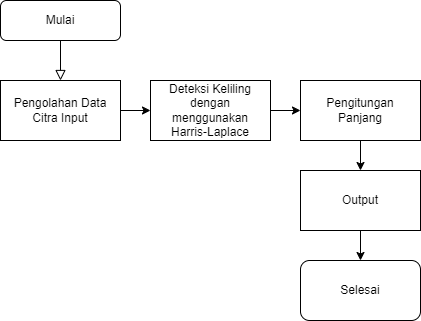
\includegraphics[width=0.45\textwidth]{gambar/Flowchart Penelitian.png}
  \caption{Diagram Penghitungan panjang ikan}
\end{figure}

\begin{figure}
  \centering{}
  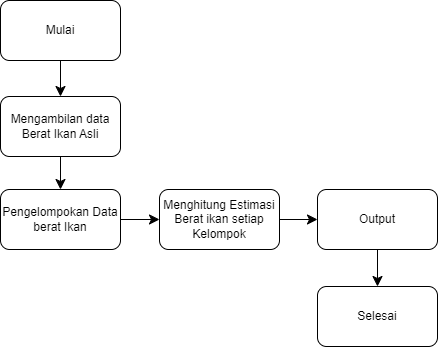
\includegraphics[width=0.45\textwidth]{gambar/Penghitungan Berat.png}
  \caption{Diagram Penghitungan berat ikan}
\end{figure}

\section{Deskripsi Sistem}

Dalam Penelitian yang akan dibuat adalah sebuah sistem yang dapat menghitung panjang serta berat rata-rata dari se-ekor ikan dengan menggunakan metode \emph{Harris-Corrner}.
Fokus dari penulis terhadap penelitian ini adalah untuk menghitung panjang serta berat rata-rata dari objek ikan. 
Citra yang digunakan oleh penulis diambil dari sebuah peternakan ikan, dimana citra tersebut akan penulis gunakan dalam pengujian sistem penghitungan panjang serta berat rata-rata ikan.

Bahasa yang penulis gunakan dalam perancangan sistem adalah Python 3. 
Tujuan penelitian adalah mendapatkan hasil perhitungan panjang dan berat ikan secara komputasi yang mana dihasilkan panjang dan berat ikan dari sebuah citra ikan. 

Tahapan yang akan diproses dalam penghitungan berat dan panjang ikan dengan menggunakan \emph{Harris-corner} adalah memasukan atau menginput citra ikan, lalu mendeteksi korner dari ikan menggunakan \emph{Harris-corner} dan menghitung panjang serta berat ikan mengunakan korner hasil dari \emph{Harris-corner}. 




% %!TEX root = ./template-skripsi.tex
%-------------------------------------------------------------------------------
%                            	BAB IV
%               		KESIMPULAN DAN SARAN
%-------------------------------------------------------------------------------

\chapter{UJI COBA DAN HASIL UJI COBA}

\section{Uji Coba}
Uji coba sistem dilakukan terhadap 30 responden anggota KOPMA UNJ dengan rincian, \textit{admin} yang terdiri dari 2 responden, pengawas yang terdiri dari 3 responden, dan anggota yang terdiri dari 25 responden. Setiap responden akan melakukan uji coba terhadap sistem yang dibuat berdasarkan peran masing-masing responden. Uji coba yang dilakukan menggunakan data dari hasil sebaran kuesioner \textit{User Acceptance Test}. \textit{User Acceptance Test} bertujuan untuk mengetahui perihal sistem yang dikembangkan apakah sudah sesuai dengan kebutuhan \textit{user} atau belum. Skala yang digunakan dalam penelitian ini adalah skala \textit{likert}.

Langkah-langkah pengujian sistem informasi Koperasi Mahasiswa Universitas Negeri Jakarta yang akan dilakukan adalah sebagai berikut:
\begin{enumerate}
	\item \textit{User} melakukan pendaftaran anggota.
	\item \textit{Admin} melakukan verifikasi penerimaan anggota.
	\item \textit Seluruh \textit{user} dapat mengelola biodata pribadi.
	\item \textit{Admin} mengelola status keanggotaan setiap \textit{user} (\textit{admin}, pengawas, atau anggota biasa).
	\item Anggota dan pengawas yang sudah memiliki akun dapat mengakses ke dalam sistem sesuai berandanya masing-masing.
	\item \textit{Admin} menambahkan data barang, stok, simpanan, transaksi anggota, dan keuangan.
	\item Data yang \textit{admin} tambahkan akan muncul dan dapat dilihat di beranda semua \textit{user}.
	\item \textit{Admin} mengelola (sunting dan hapus) data barang, stok, simpanan, transaksi anggota, dan keuangan.
	\item Data yang \textit{admin} kelola akan berubah dan dapat dilihat di beranda semua \textit{user}.	
	\item Pengawas menambahkan data penilaian untuk KOPMA UNJ.
	\item Data yang pengawas tambahkan akan muncul dan dapat dilihat di beranda  semua \textit{user}.
	\item Pengawas mengelola (sunting dan hapus) data penilaian untuk KOPMA UNJ.
	\item Data yang pengawas kelola akan berubah dan dapat dilihat di beranda semua \textit{user}.	
\end{enumerate}

Fitur milik setiap \textit{user} yang akan diuji pada sistem informasi Koperasi Mahasiswa Universitas Negeri Jakarta adalah sebagai berikut:

\begin{itemize}
	\item \textit{Admin}
	\begin{enumerate}
		\item Masuk ke dalam sistem
		\item Penyuntingan data pribadi
		\item Pengelolaan anggota (tambah, kesesuaian \textit{id}, detail, pemutihan, sunting, \textit{reset password}, tambah periode, pengelompokan, pemulihan, keuangan anggota, dan cetak)
		\item Pengelolaan barang (tambah, sunting, hapus, cetak, dan pengelompokan)
		\item Pengelolaan stok (tambah, hapus, dan cetak)
		\item Pengelolaan simpanan (tambah, hapus, cetak, dan pengelompokan)
		\item Pengelolaan transaksi (tambah, hapus, dan cetak)
		\item Transparansi penilaian
		\item Pengelolaan dan kesesuaian arus keuangan (tambah dana tambahan dan beban lain)
		\item Pengelolaan \textit{admin} (tambah dan hapus \textit{admin})
		\item Pengelolaan pengawas (tambah dan hapus pengawas)
		\item Pengelolaan penerimaan anggota (terima dan tolak anggota)
		\item Keluar dari sistem
	\end{enumerate}

	\item Anggota
	\begin{enumerate}
		\item Melakukan pendaftaran
		\item Masuk ke dalam sistem
		\item Penyuntingan data pribadi
		\item Transparansi data (barang, stok, transaksi, penilaian, dan arus keuangan)
		\item Keluar dari sistem
	\end{enumerate}
	
	\item Pengawas
	\begin{enumerate}
		\item Masuk ke dalam sistem
		\item Penyuntingan data pribadi
		\item Transparansi data (barang, stok, transaksi, dan arus keuangan)
		\item Pengelolaan penilaian (tambah, sunting, hapus, dan cetak)
		\item Keluar dari sistem
		\end{enumerate}
	\end{itemize}

Semua fitur yang diuji memiliki penilaian yang dirincikan menjadi beberapa kategori. Data kuantitatif akan dianalisis dengan menggunakan skala \textit{ likert}. Berikut kategori dan skor penilaian dalam tahap pengujian\textit{ User Acceptance Test} pada sistem informasi Koperasi Mahasiswa Universitas Negeri Jakarta dengan menggunakan skala \textit{likert}:\\

\begin{tabular}{lll}
SS& = Sangat Setuju& diberikan nilai 5\\
S& = Setuju& diberikan nilai 4\\
C& = Cukup& diberikan nilai 3\\
TS& = Tidak Setuju& diberikan nilai 2\\
STS& = Sangat Tidak Setuju& diberikan nilai 1\\
\\
\end{tabular}

Kemudian hasil pendataan yang telah didapatkan dengan teknik penyebaran angket dikalkulasikan dengan menggunakan sistem penilaian sebagai berikut:

\begin{itemize}
	\item Nilai total
	
	Nilai total merupakan nilai dari hasil perhitungan antara responden kuesioner angket dengan nilai di setiap poin pertanyaan. Berikut merupakan rumus nilai total:
	
	\textit{Nilai total = jumlah nilai setiap soal}
	
	\item Nilai rata-rata
	
	Nilai rata-rata merupakan nilai dari hasil perhitungan antara nilai total dengan jumlah responden yang mengisi kuesioner angket. Berikut merupakan rumus dari nilai rata-rata:

	\textit{Nilai rata-rata = nilai total / jumlah responden}
	
\end{itemize}

Untuk mengetahui kualitas produk yang dikembangkan layak atau tidak, maka perlu ditentukan dengan menghitung seluruh nilai rata-rata dari setiap pertanyaan. Nilai tersebut kemudian akan dibandingkan dengan interpretasi skor pada skala \textit{likert}. Analisis data yang disajikan ke distribusi skor dan persentase terhadap kategori menggunakan interpretasi skor untuk skala \textit{likert}. Berikut rentang interpretasi skor untuk skala \textit{likert}:\\

\begin{tabular}{lll}
	Nilai& = 0\% - 20\%& Sangat Kurang Sesuai \\
	Nilai& = 21\% - 40\%& Kurang Sesuai\\
	Nilai& = 41\% - 60\%& Cukup Sesuai\\
	Nilai& = 61\% - 80\%& Sesuai\\
	Nilai& = 81\% - 100\%& Sangat Sesuai\\
\end{tabular}

\section{Hasil Uji Coba}
Berdasarkan hasil uji coba \textit{User Acceptance Test} yang dilakukan terhadap 30 anggota KOPMA UNJ, yakni \textit{admin} yang terdiri dari 2 responden, pengawas terdiri dari 3 responden, dan anggota terdiri dari 25 responden, diperoleh hasil uji coba sebagai berikut:

\subsection{\textit{Admin}}
Berikut merupakan daftar pertanyaan \textit{User Acceptance Test} pada \textit{Admin}:

\begin{table}[H]
	\centering
	\caption{Daftar Pertanyaan \textit{User Acceptance Test} pada \textit{Admin}}
	\includegraphics[width=1.0\textwidth]{gambar/Tabel_Admin1}
\end{table}

\begin{table}[H]
	\centering
	\caption{Daftar Pertanyaan \textit{User Acceptance Test} pada \textit{Admin}}
	\includegraphics[width=1.0\textwidth]{gambar/Tabel_Admin2}
\end{table}

Setelah kuisioner \textit{admin} diberikan kepada responden, kemudian data kuesioner diolah untuk mendapatkan hasil penilaian \textit{user acceptance test}. Adapun hasil penilaian \textit{user acceptance test} tersebut yaitu:

\begin{table}[H]
	\centering
	\caption{Data Hasil Penyebaran Kuesioner \textit{User Acceptance Test} pada \textit{Admin}}
	\includegraphics[width=1\textwidth]{gambar/Hasil_Admin}
\end{table}

Dari hasil penilaian pengujian \textit{user acceptance test} dapat diambil kesimpulan yaitu:

\begin{enumerate}
	\item Pengguna sistem yang telah memilih Sangat Tidak Setuju (STS) memiliki persentase 0\%
	\item Pengguna sistem yang telah memilih Tidak Setuju (TS) memiliki persentase 0\%
	\item Pengguna sistem yang telah memilih Cukup (C) memiliki persentase 8\%.
	\item Pengguna sistem yang telah memilih Setuju (S) memiliki persentase 57\%.
	\item Pengguna sistem yang telah memilih Sangat Setuju (SS) memiliki persentase 35\%.
	\item Rata-rata penerimaan \textit{user} adalah 4,27 dari 5 atau sekitar 85\%.
\end{enumerate}

\begin{figure}[H]
	\centering
	\includegraphics[width=1\textwidth]{gambar/Grafik_Admin}
	\caption{Grafik Hasil Penyebaran Kuesioner \textit{User Acceptance Test} pada \textit{Admin}}
\end{figure}

Berdasarkan hasil pengujian \textit{user acceptance test} yang diujikan kepada 2 responden \textit{admin}, dapat dilihat bahwa secara keseluruhan 35\% menjawab sangat setuju, 57\% menjawab setuju, 8\% menjawab cukup, serta rata-rata penerimaan \textit{user} terhadap kesesuaian sistem dengan kebutuhan adalah 4,27 dari 5 atau sekitar 85\%, oleh karena itu dapat diambil kesimpulan bahwa fitur yang \textit{admin} butuhkan dalam sistem informasi yang dirancang sudah sangat sesuai dengan kebutuhan dan berjalan dengan baik.  

\subsection{\textit{Anggota}}
Berikut merupakan daftar pertanyaan \textit{User Acceptance Test} pada Anggota

\begin{table}[H]
	\centering
	\caption{Daftar Pertanyaan \textit{User Acceptance Test} pada Anggota}
	\includegraphics[width=1\textwidth]{gambar/Tabel_Anggota}
\end{table}

Setelah kuisioner anggota diberikan kepada responden, kemudian data kuesioner diolah untuk mendapatkan hasil penilaian \textit{user acceptance test}. Adapun hasil penilaian \textit{user acceptance test} tersebut yaitu:

\begin{table}[H]
	\centering
	\caption{Data Hasil Penyebaran Kuesioner \textit{User Acceptance Test} pada Anggota}
	\includegraphics[width=1\textwidth]{gambar/Hasil_Anggota}
\end{table}

Dari hasil pengujian \textit{user acceptance test} dapat diambil kesimpulan yaitu:

\begin{enumerate}
	\item Pengguna sistem yang telah memilih Sangat Tidak Setuju (STS) memiliki persentase 0\%
	\item Pengguna sistem yang telah memilih Tidak Setuju (TS) memiliki persentase 0\%
	\item Pengguna sistem yang telah memilih Cukup (C) memiliki persentase 23\%.
	\item Pengguna sistem yang telah memilih Setuju (S) memiliki persentase 58\%.
	\item Pengguna sistem yang telah memilih Sangat Setuju (SS) memiliki persentase 19\%.
	\item Rata-rata penerimaan \textit{user} adalah 3,96 dari 5 atau sekitar 79\%.
\end{enumerate}

\begin{figure}[H]
	\centering
	\includegraphics[width=1\textwidth]{gambar/Grafik_Anggota}
	\caption{Grafik Hasil Penyebaran Kuesioner \textit{User Acceptance Test} pada Anggota}
\end{figure}

Berdasarkan hasil pengujian \textit{user acceptance test} yang diujikan kepada 25 responden anggota, dapat dilihat bahwa secara keseluruhan 19\% menjawab sangat setuju, 58\% menjawab setuju, 23\% menjawab cukup, serta rata-rata penerimaan \textit{user} terhadap kesesuaian sistem dengan kebutuhan adalah 3,96 dari 5 atau sekitar 79\%, oleh karena itu dapat diambil kesimpulan bahwa fitur yang anggota butuhkan dalam sistem informasi yang dirancang sudah sesuai dengan kebutuhan dan berjalan dengan baik. 
\\
\\
\\
\\
\\

\subsection{\textit{Pengawas}}
Berikut merupakan daftar pertanyaan \textit{User Acceptance Test} pada Pengawas

\begin{table}[H]
	\centering
	\caption{Daftar Pertanyaan \textit{User Acceptance Test} pada Pengawas}
	\includegraphics[width=1\textwidth]{gambar/Tabel_Pengawas}
\end{table}

Setelah kuisioner pengawas diberikan kepada responden, kemudian data kuesioner diolah untuk mendapatkan hasil penilaian \textit{user acceptance test}. Adapun hasil penilaian \textit{user acceptance test tersebut} tersebut yaitu:

\begin{table}[H]
	\centering
	\caption{Data Hasil Penyebaran Kuesioner \textit{User Acceptance Test} pada Pengawas}
	\includegraphics[width=1\textwidth]{gambar/Hasil_Pengawas}
\end{table}

Dari hasil penilaian pengujian \textit{user acceptance test} dapat diambil kesimpulan yaitu:

\begin{enumerate}
	\item Pengguna sistem yang telah memilih Sangat Tidak Setuju (STS) memiliki persentase 0\%
	\item Pengguna sistem yang telah memilih Tidak Setuju (TS) memiliki persentase 0\%
	\item Pengguna sistem yang telah memilih Cukup (C) memiliki persentase 2\%.
	\item Pengguna sistem yang telah memilih Setuju (S) memiliki persentase 42\%.
	\item Pengguna sistem yang telah memilih Sangat Setuju (SS) memiliki persentase 56\%.
	\item Rata-rata penerimaan \textit{user} adalah 4,53 dari 5 atau sekitar 91\%.
\end{enumerate}

\begin{figure}[H]
	\centering
	\includegraphics[width=1\textwidth]{gambar/Grafik_Pengawas}
	\caption{Grafik Hasil Penyebaran Kuesioner \textit{User Acceptance Test} pada Pengawas}
\end{figure}

Berdasarkan hasil pengujian \textit{user acceptance test} yang diujikan kepada 3 responden pengawas, dapat dilihat bahwa secara keseluruhan 56\% menjawab sangat setuju, 42\% menjawab setuju, 2\% menjawab cukup, serta rata-rata penerimaan \textit{user} terhadap kesesuaian sistem dengan kebutuhan adalah 4,53 dari 5 atau sekitar 91\%, oleh karena itu dapat diambil kesimpulan bahwa fitur yang pengawas butuhkan dalam sistem informasi yang dirancang sudah sangat sesuai dengan kebutuhan dan berjalan dengan baik. 

% Baris ini digunakan untuk membantu dalam melakukan sitasi
% Karena diapit dengan comment, maka baris ini akan diabaikan
% oleh compiler LaTeX.
\begin{comment}
\bibliography{daftar-pustaka}
\end{comment}

% %!TEX root = ./template-skripsi.tex
%-------------------------------------------------------------------------------
%                            	BAB IV
%               		KESIMPULAN DAN SARAN
%-------------------------------------------------------------------------------

\chapter{KESIMPULAN DAN SARAN}

\section{Kesimpulan}
Berdasarkan hasil implementasi dan pengujian fitur sistem informasi yang telah dirancang, maka diperoleh kesimpulan sebagai berikut:

\begin{enumerate}
	\item Perancangan sistem informasi operasi serba usaha berbasis \emph{website} pada lembaga Koperasi Mahasiswa Universitas Negeri Jakarta menggunakan metode pengembangan perangkat lunak \textit{System Development Life Cycle} dengan \textit{spiral model} yang memiliki beberapa tahapan, yaitu analisis kebutuhan, perancangan desain sistem \textit{(prototype)}, pengimplementasian (\textit{coding \& testing-unit}), dan \textit{maintenance} (umpan balik dan tanggapan).
	
	\item Sistem informasi Koperasi Mahasiswa Universitas Negeri Jakarta dibangun dengan menggunakan \textit{framework codeigniter} dan \textit{framework bootstrap}. \textit{Codeigniter} untuk membangun sisi dalam \textit{back-end} dan \textit{Bootstrap} yang mempercantik bagian luar \textit{front-end}. Berdasarkan pengolahan data hasil kuesioner \textit{user acceptance test}, didapatkan rata-rata persentase mencapai angka 4,27 dari 5 atau sekitar 85\% untuk \textit{admin} yang berarti sistem sudah sangat sesuai, 3,96 dari 5 atau sekitar 79\% untuk anggota yang berarti sistem sudah sesuai, dan 4,53 dari 5 atau sekitar 91\% pada sistem pengawas yang berarti sistem sudah sangat sesuai.
	
	\item Sistem informasi Koperasi Mahasiswa Universitas Negeri Jakarta berbasis \textit{website} dibangun agar sistem pengelolaan data di KOPMA UNJ dapat menjadi lebih efektif dan efisian, serta agar kemungkinan adanya \textit{human error} dapat diatasi. Data yang dikelola berupa data anggota, barang, stok (pergudangan), simpanan, transaksi, penilaian, dan keuangan.
	
	\item Sistem informasi Koperasi Mahasiswa Universitas Negeri Jakarta berbasis \textit{website} mempermudah \textit{admin} dalam melakukan pengelolaan data yang ada di KOPMA UNJ, mempermudah pengawas dalam melakukan pengelolaan data penilan, dan membuat anggota dapat mengetahui transparansi simpanan yang mereka bayarkan hingga mengetahui transparansi sisa hasil usaha yang mereka dapatkan.
\end{enumerate}

\section{Saran}
Adapun saran untuk penelitian selanjutnya adalah:
\begin{enumerate} 
	\item Mengintegrasikan sistem informasi KOPMA UNJ dengan aplikasi dan sistem \textit{scanning barcode} agar proses transaksi semakin efektif dan efisien.
	\item Menambahkan dan mengintegrasikan sistem informasi KOPMA UNJ dengan aplikasi untuk \textit{scanning barcode} pada kartu anggota agar proses kebutuhan simpanan dan transaksi untuk anggota dapat semakin efektif dan efisien.
	\item Menambahkan sistem pengelolaan kegiatan keorganisasian KOPMA UNJ yang merupakan bagian dari peran KOPMA UNJ sebagai Organisasi Kemahasiswaan di UNJ.
	\item Membuat pengembangan sistem informasi KOPMA UNJ berbasis \textit{mobile} (\textit{android}).
\end{enumerate}


% Baris ini digunakan untuk membantu dalam melakukan sitasi
% Karena diapit dengan comment, maka baris ini akan diabaikan
% oleh compiler LaTeX.
\begin{comment}
\bibliography{daftar-pustaka}
\end{comment}


%-----------------------------------------------------------------
%Disini akhir masukan Bab
%-----------------------------------------------------------------


%-----------------------------------------------------------------
% Disini awal masukan untuk Daftar Pustaka
% - Daftar pustaka diambil dari file .bib yang ada pada folder ini
%   juga.
% - Untuk memudahkan dalam memanajemen dan menggenerate file .bib
%   gunakan reference manager seperti Mendeley, Zotero, EndNote,
%   dll.
%-----------------------------------------------------------------
% \bibliography{daftar-pustaka}
% \bibliographystyle{apalike}
\onehalfspacing{}
\addcontentsline{toc}{chapter}{DAFTAR PUSTAKA}
% \singlespacing{}
\printbibliography{}
%-----------------------------------------------------------------
%Disini akhir masukan Daftar Pustaka
%-----------------------------------------------------------------


\end{document}
